\section{Project Charter}

The Project Charter was developed at the conclusion of the planning phase, rather than at the beginning. This choice was intentional: by first completing the full breakdown of tasks, structure, scheduling, and resource analysis, the scope and objectives of the project became clearer and more grounded in the actual complexity of the work. Defining the charter retrospectively allowed for a more accurate and comprehensive summary of the project’s boundaries and key deliverables.

This approach also ensured alignment between the strategic goals and the operational details identified throughout the planning process. The finalized charter consolidates the refined understanding of stakeholders, constraints and success criteria, effectively bridging theoretical planning tools with the practical needs of project execution.

The complete project charter can be found in the attachments.

INSERIRE REFERENCE AL DOCUMENTO QUI

\section{Scope Definition and WBSs}

The scope of the project covers the complete lifecycle of an industrial system, from initial process engineering through procurement, construction, and testing of the final assembly.
The final objective is the end-to-end delivery of a reverse osmosis desalination skid for offshore use, designed to provide 20 m³/day of potable water for 90 personnel, in compliance with WHO and IECEx standards.

The scope includes engineering, procurement, assembly, FAT with third-party certification, and full documentation delivery.
Out of scope are post-deployment activities, such as on-site integration, operational training, and long-term maintenance, which are assumed to be managed in a separate phase by the client.

The scope was defined through a detailed decomposition using three alternative Work Breakdown Structures:
\begin{itemize}
    \item \textbf{WBS1: Phase-Oriented}
          Organizes activities sequentially by project phases: Engineering, Procurement, Construction, and Testing.
    \item \textbf{WBS2: System-Oriented}
          Structures the work according to functional systems: Process, Piping, Structural, and Electrical and Control.
    \item \textbf{WBS3: Location-Oriented}
          Breaks down the project by physical modules: Skid Frame, Piping Module, Process Equipment Zone, and Control and Instrumentation Panel.
\end{itemize}
Although WBS2 was regarded as more professional, WBS1 was selected to enable a simpler and more linear execution of the project, taking into account the team’s relatively limited experience in this area.
All three WBS can be found in the attachments.

INSERIRE REFERENCE QUI

The project includes approximately 70 interconnected activities, each linked by defined precedencies.
Each Work Package (WP) includes:
\begin{itemize}
    \item \textbf{Estimated duration and required resources}
          Each work package specifies the expected time frame for completion and details the human, material, and financial resources necessary for execution.
    \item \textbf{Logical dependencies enabling scheduling and critical path identification}
          Predecessor and successor relationships are defined for each work package, supporting the development of the project schedule and identification of the critical path.
\end{itemize}

\section{Organizational Breakdown Structure (OBS)}

The Organizational Breakdown Structure (OBS) was developed to define the distribution of responsibilities and to ensure accountability throughout all the phases of the project. It complements the Work Breakdown Structure by mapping each work package or group of activities to the organizational units responsible for their execution.

Out of the project stakeholders we identified in the project charter, the following were left out of the OBS:
\begin{itemize}
    \item Sponsor: while finances the project, is not involved in its development.
    \item Customer Representative: communicates with the project manager but doesn't have a formal hierarchical position.
    \item Certifying Body: contributes to the project but is not part of the organization.
\end{itemize}

Each WBS element was cross-referenced with the OBS to clarify ownership and facilitate delegation of responsibilities. This linkage supports not only planning but also later phases of project control, risk management, and change handling.

By aligning the WBS with the OBS ~\ref{fig:obs}, we ensured that all deliverables have a designated owner and that no scope elements are left unassigned, an essential condition for effective execution in a complex multidisciplinary project environment.

The crossing between OBS and WBS is included in the attachments.

\begin{figure}[p]
    \centering
    \rotatebox{90}{%
        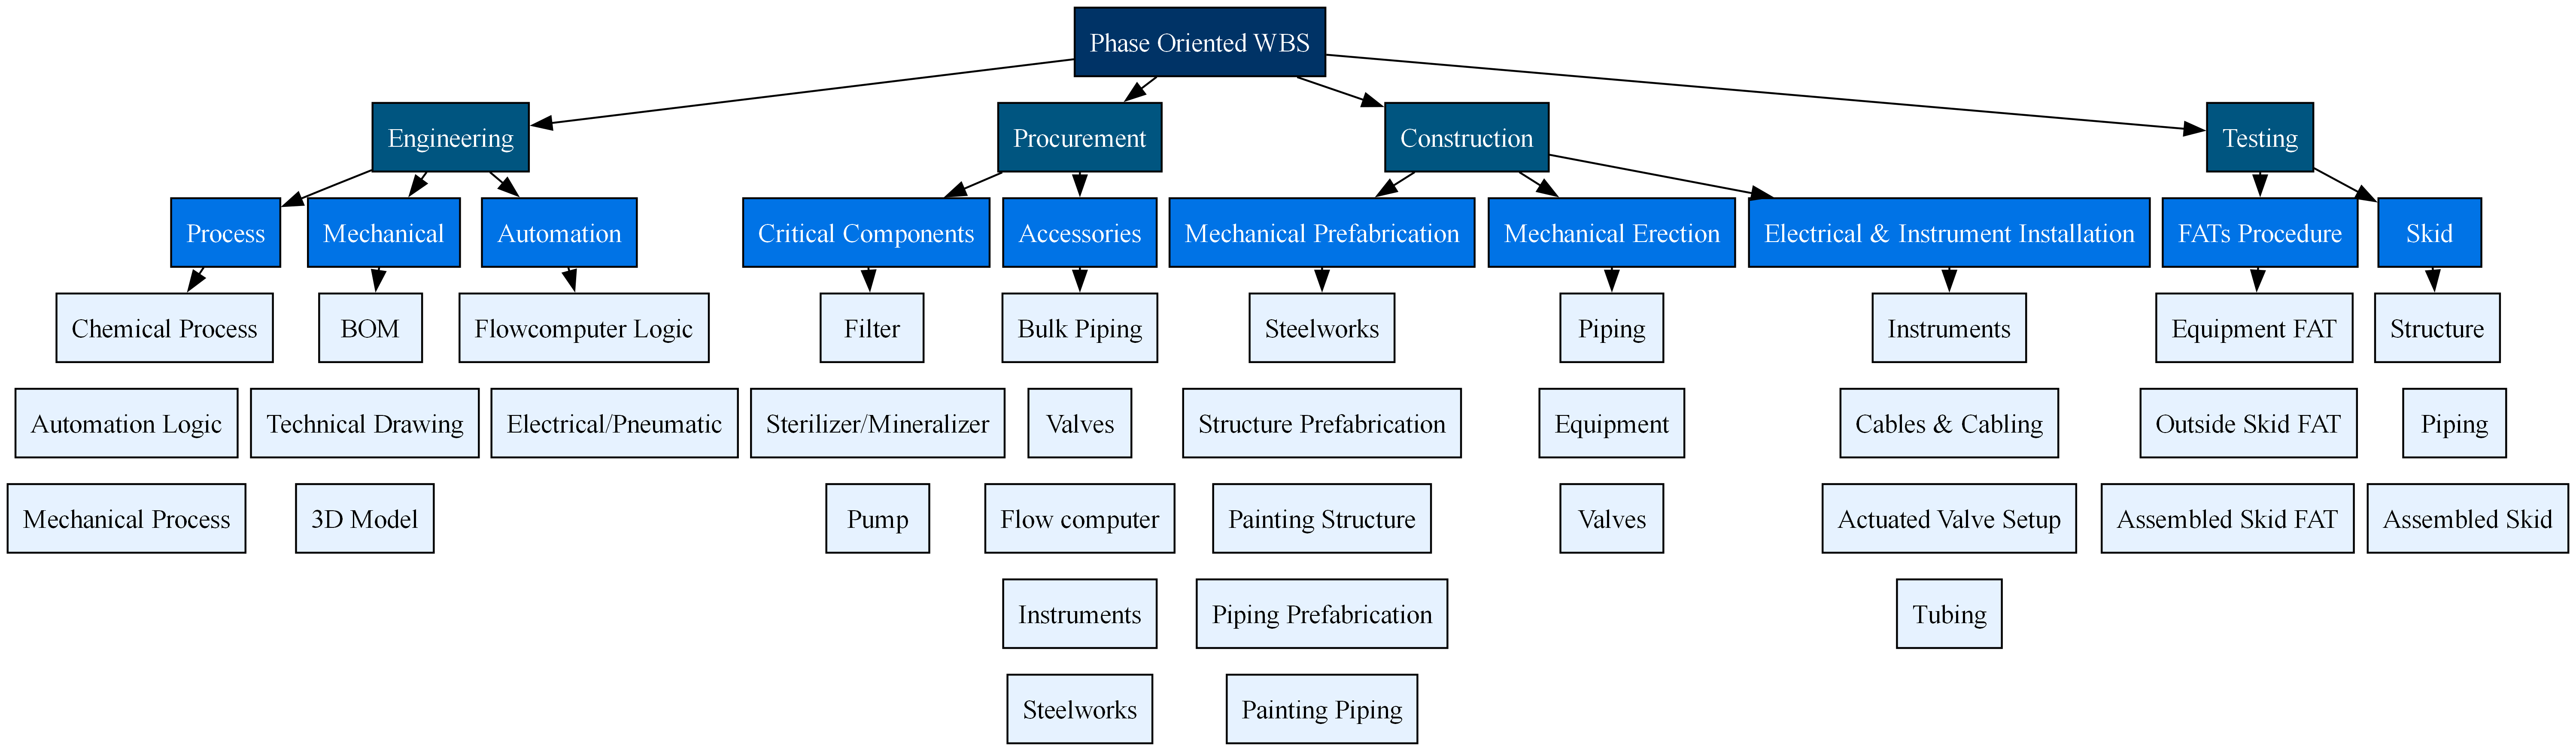
\includegraphics[width=0.95\textheight,keepaspectratio]{../WBS1.png}
    }
    \caption{Selected Phase-Oriented Work Breakdown Structure (WBS1) for the project.}
    \label{fig:wbs1}
\end{figure}

\section{Work Package Description}

Each work package (WP) in the project represents a self-contained unit of work with clearly defined deliverables, responsible parties, resource allocations, and dependencies. The WP structure was derived from the WBS and refined to ensure completeness and traceability in both scheduling and cost estimation.

The purpose of this section is to present a standardized overview of selected work packages that cover the major functional and temporal segments of the project. This degree of detail ensures clarity in execution, aids progress tracking, and allows efficient allocation of both human and material resources.

The following template has been adopted for the WP description:

WP Name: [Insert Work Package Title AND CODE]
Description:
[Brief explanation of the objective and scope of the WP]

Estimated Duration: [e.g., 10 working days]

Resources Involved:
\begin{itemize}
    \item External Engineering: [e.g., 2 engineers for 10 days]
    \item Internal Engineering: [e.g., 1 engineer for 10 days]
    \item Materials: [e.g., €xxx for materials]
    \item Supplier: [e.g., €xxx for supplier services]
\end{itemize}

Dependencies:
[List of predecessor WPs or milestones]

Responsible Unit (OBS): [e.g., Engineering Department]

Risks / Notes:
[Any known issues, constraints, or risk considerations]

WP Name: PFD - Heat and Mass Balance
Description:
Defines process flow and thermodynamic balances of the system.

Estimated Duration: 13 working days

Resources Involved:
\begin{itemize}
    \item External Engineering: 2,500.00€ for engineering services
\end{itemize}

Dependencies:
No Predecessor

Responsible Unit (OBS): Technical Manager

Risks / Notes:
As the initial Work Package, any delay at this stage will have a cascading impact on all downstream engineering and procurement activities.

WP Name: 3D Model
Description:
Full 3D representation of skid layout and components.

Estimated Duration: 20 working days

Resources Involved:
\begin{itemize}
    \item External Engineering: 6,000.00€ for engineering services
\end{itemize}

Dependencies:
P\ and ID

Responsible Unit (OBS): Technical Manager

Risks / Notes:
This WP enables the issuance of key construction documents. It relies on accurate input from equipment engineering and procurement, particularly regarding dimensions, weights, and service access requirements. Supplier delays may compromise the model’s accuracy and disrupt project flow.

WP Name: Pump Procurement
Description:
Purchasing of pump equipment.

Estimated Duration: 150 working days

Resources Involved:
\begin{itemize}
    \item  Supplier 7.000,00€
\end{itemize}

Dependencies:
Filter Data Sheet

Responsible Unit (OBS): Package Manager

Risks / Notes:
Delays in receiving the final Filter Data Sheet may postpone pump selection and ordering.
Inaccurate or incomplete specifications can lead to mismatched selections and require costly rework.
The long supplier lead time (150 working days) makes schedule adherence critical.
Early engagement with the vendor is essential to manage documentation, certifications, and delivery logistics.
Coordination with the 3D design team is required to ensure spatial compatibility with the skid layout and utilities.

WP Name: Structures Prefabrication
Description:
Assembly of structural steel components.

Estimated Duration: 5 working days

Resources Involved:
\begin{itemize}
    \item  Internal Manpower : 4 people @ 50€/hr (for this project)
\end{itemize}

Dependencies:
Structures DWG; Steelworks\ and support Material Procurement

Responsible Unit (OBS): WorkShop Manager

Risks / Notes:
This Work Package initiates the construction phase and may serve as a milestone for the second client invoicing. Timely availability of drawings and steel materials is critical to avoid disruption of workshop activities.

WP Name: Final Tests
Description:
Full system validation and compliance tests.

Estimated Duration: 1 working day

Resources Involved:
\begin{itemize}
    \item  Internal Manpower : 4 people @ 50€/hr (for this project)
    \item  Third Party : 3,000€ for Certifying Services

\end{itemize}

Dependencies:
Automation Tests; Assembled Skid FAT

Responsible Unit (OBS): QC Manager

Risks / Notes:
This Work Package closes the project and includes the opportunity for formal delivery. The successful execution of tests and handover of the Documentation Pack may trigger the final invoicing to the client.

The short description for each WP can be found in the CBS attachment.

INSERIRE REFERENCE QUI

\section{Cost Estimation}

The project’s cost estimation was conducted by aggregating resource-based costs at the work package level, using data defined in the Work Breakdown Structure and refined through the Cost Breakdown Structure (CBS). Each task was associated with one or more resource categories, including:
\begin{itemize}
    \item Materials
    \item External Engineering
    \item Supplier-provided
    \item Internal Manpower
    \item Internal Engineering
\end{itemize}


These were estimated either as lump-sum values (e.g., for procurement items and subcontracted services) or time-phased allocations (e.g., for internal labor and engineering hours).

Here the cost structure is represented:

\begin{figure}[p]
    \centering
    \rotatebox{90}{%
        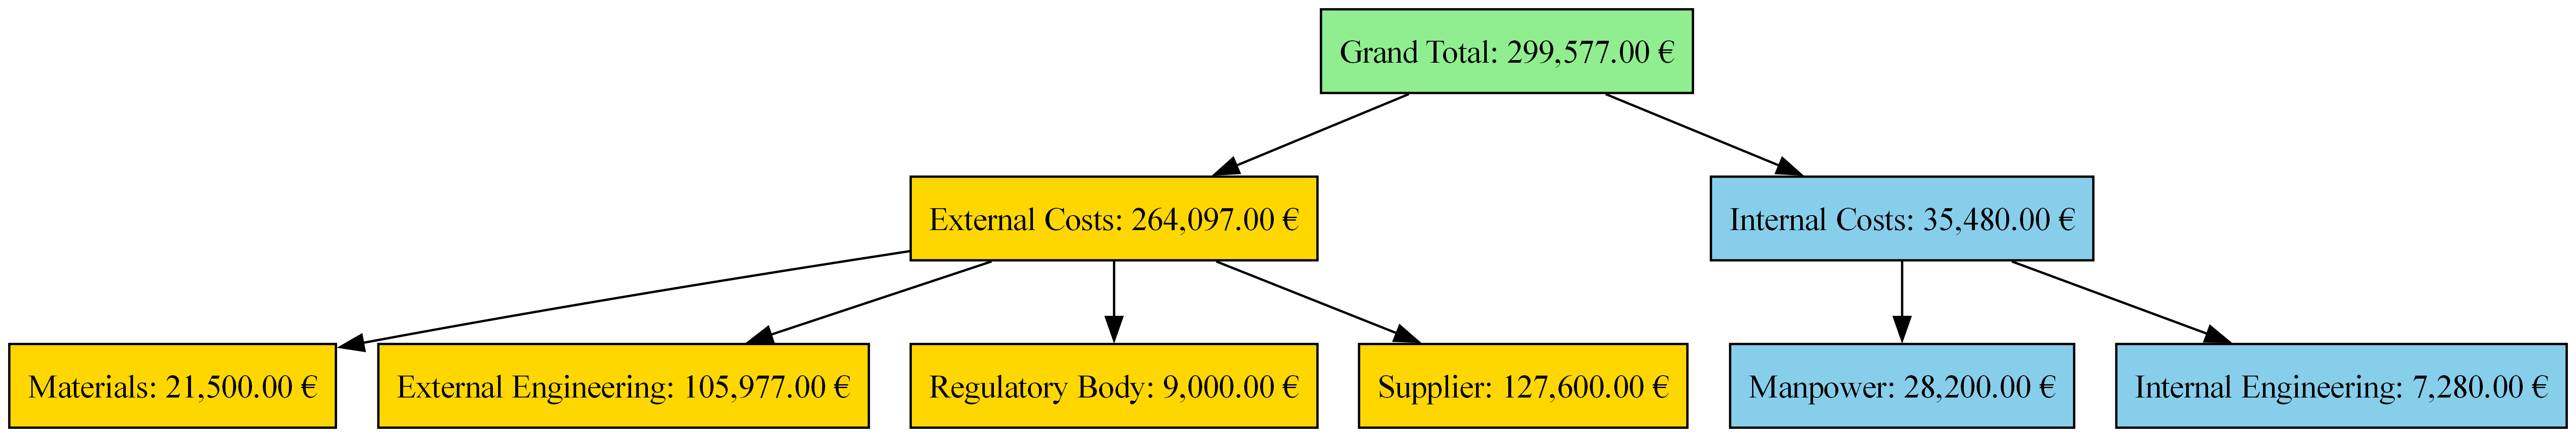
\includegraphics[width=\textwidth]{../cost_breakdown_structure.png}
    }
    \caption{Cost Structure of the project.}
    \label{fig:CS}
\end{figure}

The total projected cost of the project amounts to approximately €299,577.00, broken down into:
\begin{itemize}
    \item \textbf{Total Cost:} €299,577.00
    \item \textbf{External Costs:} €264,097.00 (approximately 89\%), covering materials, external engineering, and supplier-provided items.
    \item \textbf{Internal Costs:} €35,480.00 (approximately 11\%), covering internal manpower and internal engineering.
\end{itemize}

This distribution reflects the industrial nature of the project, where most of the value is embedded in externally sourced equipment and services.

The CBS helped validate consistency between WBS items and cost drivers, enabling cross-checks between time scheduling, deliverables, and financial expectations. Costs were also used as inputs for resource profiling, cash flow planning, and the S-curve analysis to ensure alignment across planning layers.

For the detailed cost breakdown refer to the excel file attached.

INSERIRE REFERENCE QUI

\section{Resource, Scheduling and Time Management}
\subsection{Resource definition}
Resource management in this project was structured around the identification, allocation, and time-distributed usage of five main resource categories: Materials, External Engineering, Supplier, Internal Manpower, and Internal Engineering. Each activity in the work plan was linked to one or more of these resources, with corresponding cost and workload estimates derived from realistic industrial assumptions. All resources were evaluated in terms of monetary cost.

The allocation strategy distinguishes between:
\begin{itemize}
    \item \textbf{Internal resources:} e.g., internal engineering effort, which is allocated and consumed steadily over the duration of a task, typically measured
    \item \textbf{External resources:} e.g., supplier costs, which are incurred at specific points in time, such as the start or end of the procurement phase.
\end{itemize}

\subsection{Scheduling definition}
Using the defined network of dependencies, a full forward and backward pass was executed to determine the early start (ES), early finish (EF), late start (LS), and late finish (LF) for each activity, thereby identifying the critical path and available float.

Refer to the attachments for the complete network diagram.

INSERIRE REFERENCE QUI

\subsection{Analysis and Possible optimizations}
Two scheduling strategies were compared:
\begin{itemize}
    \item \textbf{Early Start Plan:} This plan focuses on starting tasks as early as possible, thereby minimizing the overall project duration.
    \item \textbf{Late Start Plan:} This plan allows tasks to start later, potentially reducing early resource and financial exposure.
\end{itemize}

Accordingly, two different GANTT charts were developed and compared in terms of time management effectiveness and financial exposure issues.

The early start approach revealed a high financial and resource exposure during the initial and middle stages of the project. However, it also highlighted significant free float in non-critical activities, offering flexibility to optimize the allocation of resources and delay certain purchases or efforts without impacting the final delivery date.

On the other hand, the late start approach reveals the availability of enough free float to significantly impact the financial exposure, by shifting it towards the end of the project.

In a real-case scenario, effective optimization of task scheduling would be essential. The delay of specific tasks, particularly internal ones, would likely reduce early financial exposure.

The GANTT charts for the two analyzed cases can be found in the attachments.

INSERIRE REFERENCE QUI

Here follow a comparison of resource and s-curves for the two scenarios:

\begin{figure}[p]
    \begin{minipage}{\textwidth}
        \centering
        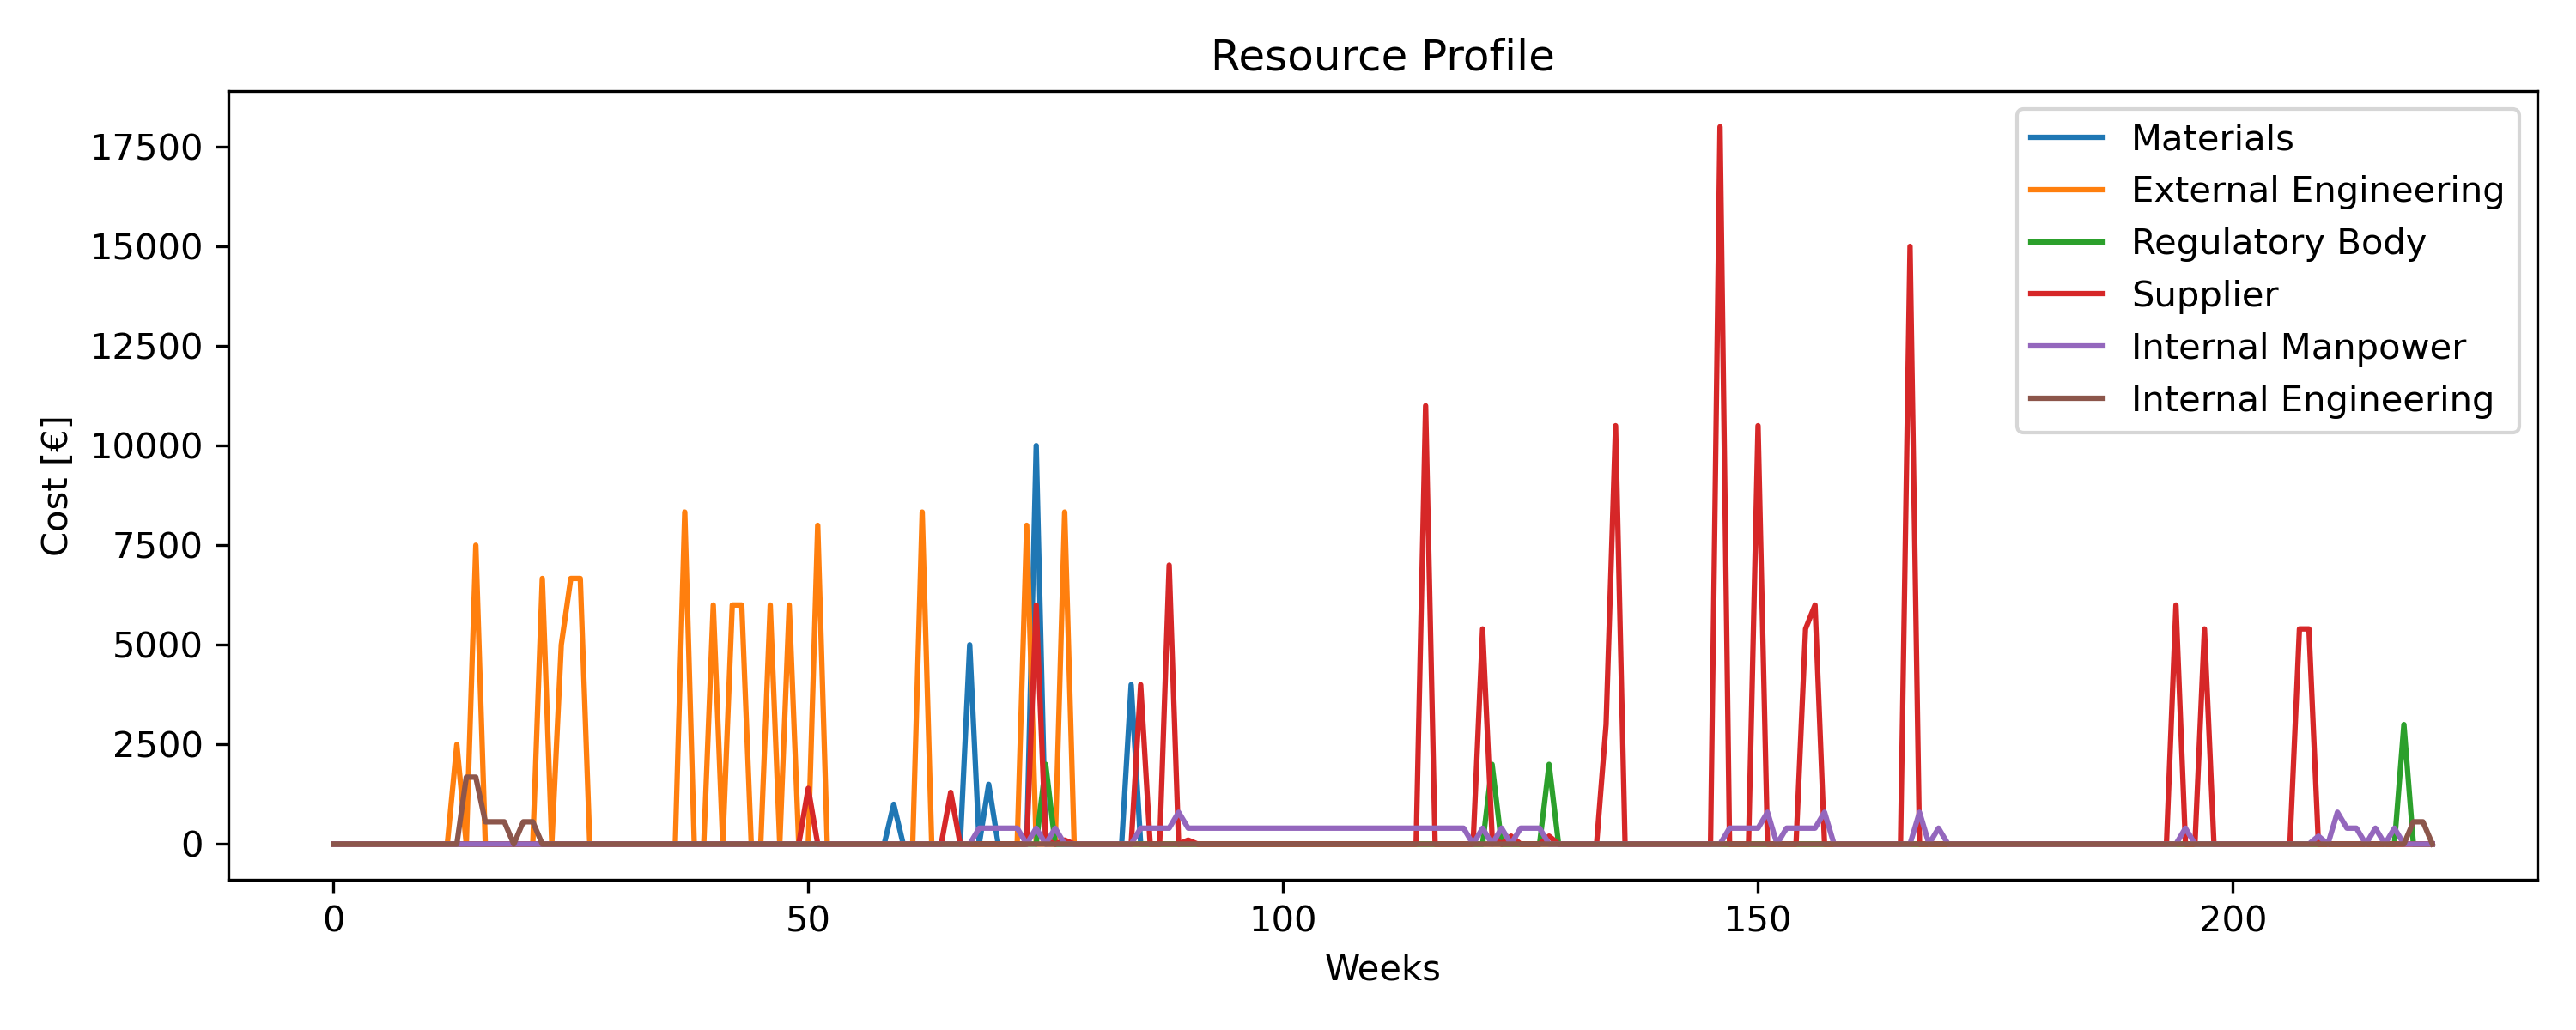
\includegraphics[width=\textwidth]{../resource_profile_E.png}
        \captionof{figure}{Resource Profile - Early Start Scenario}
        \label{fig:resource_profile_early}
    \end{minipage}\hfill
    \begin{minipage}{\textwidth}
        \centering
        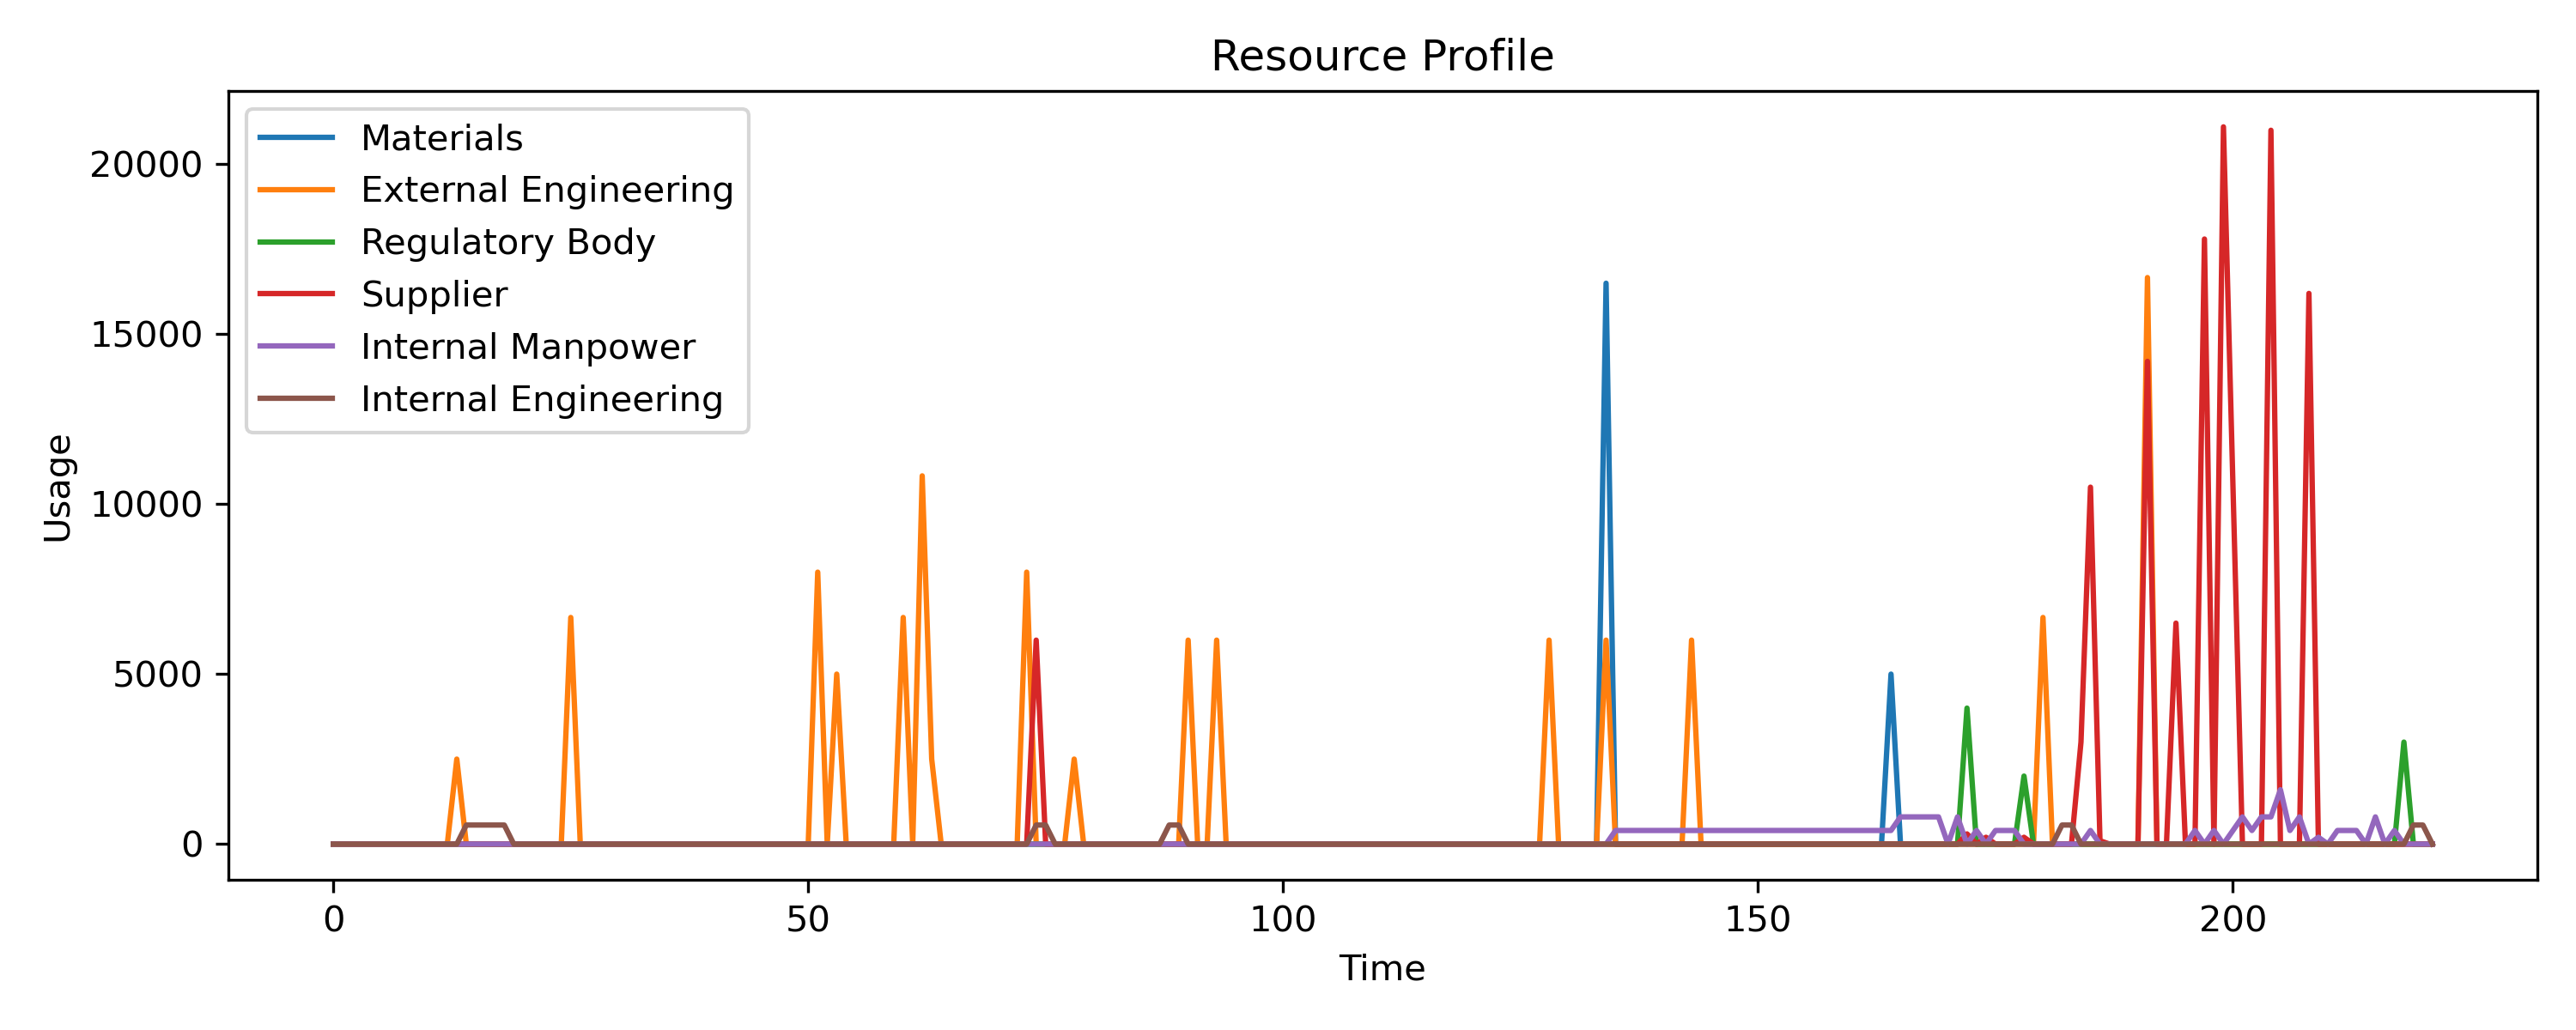
\includegraphics[width=\textwidth]{../resource_profile_L.png}
        \captionof{figure}{Resource Profile - Late Start Scenario}
        \label{fig:resource_profile_late}
    \end{minipage}
\end{figure}

\begin{figure}[p]
    \centering
            \begin{minipage}{\textwidth}
        \centering
        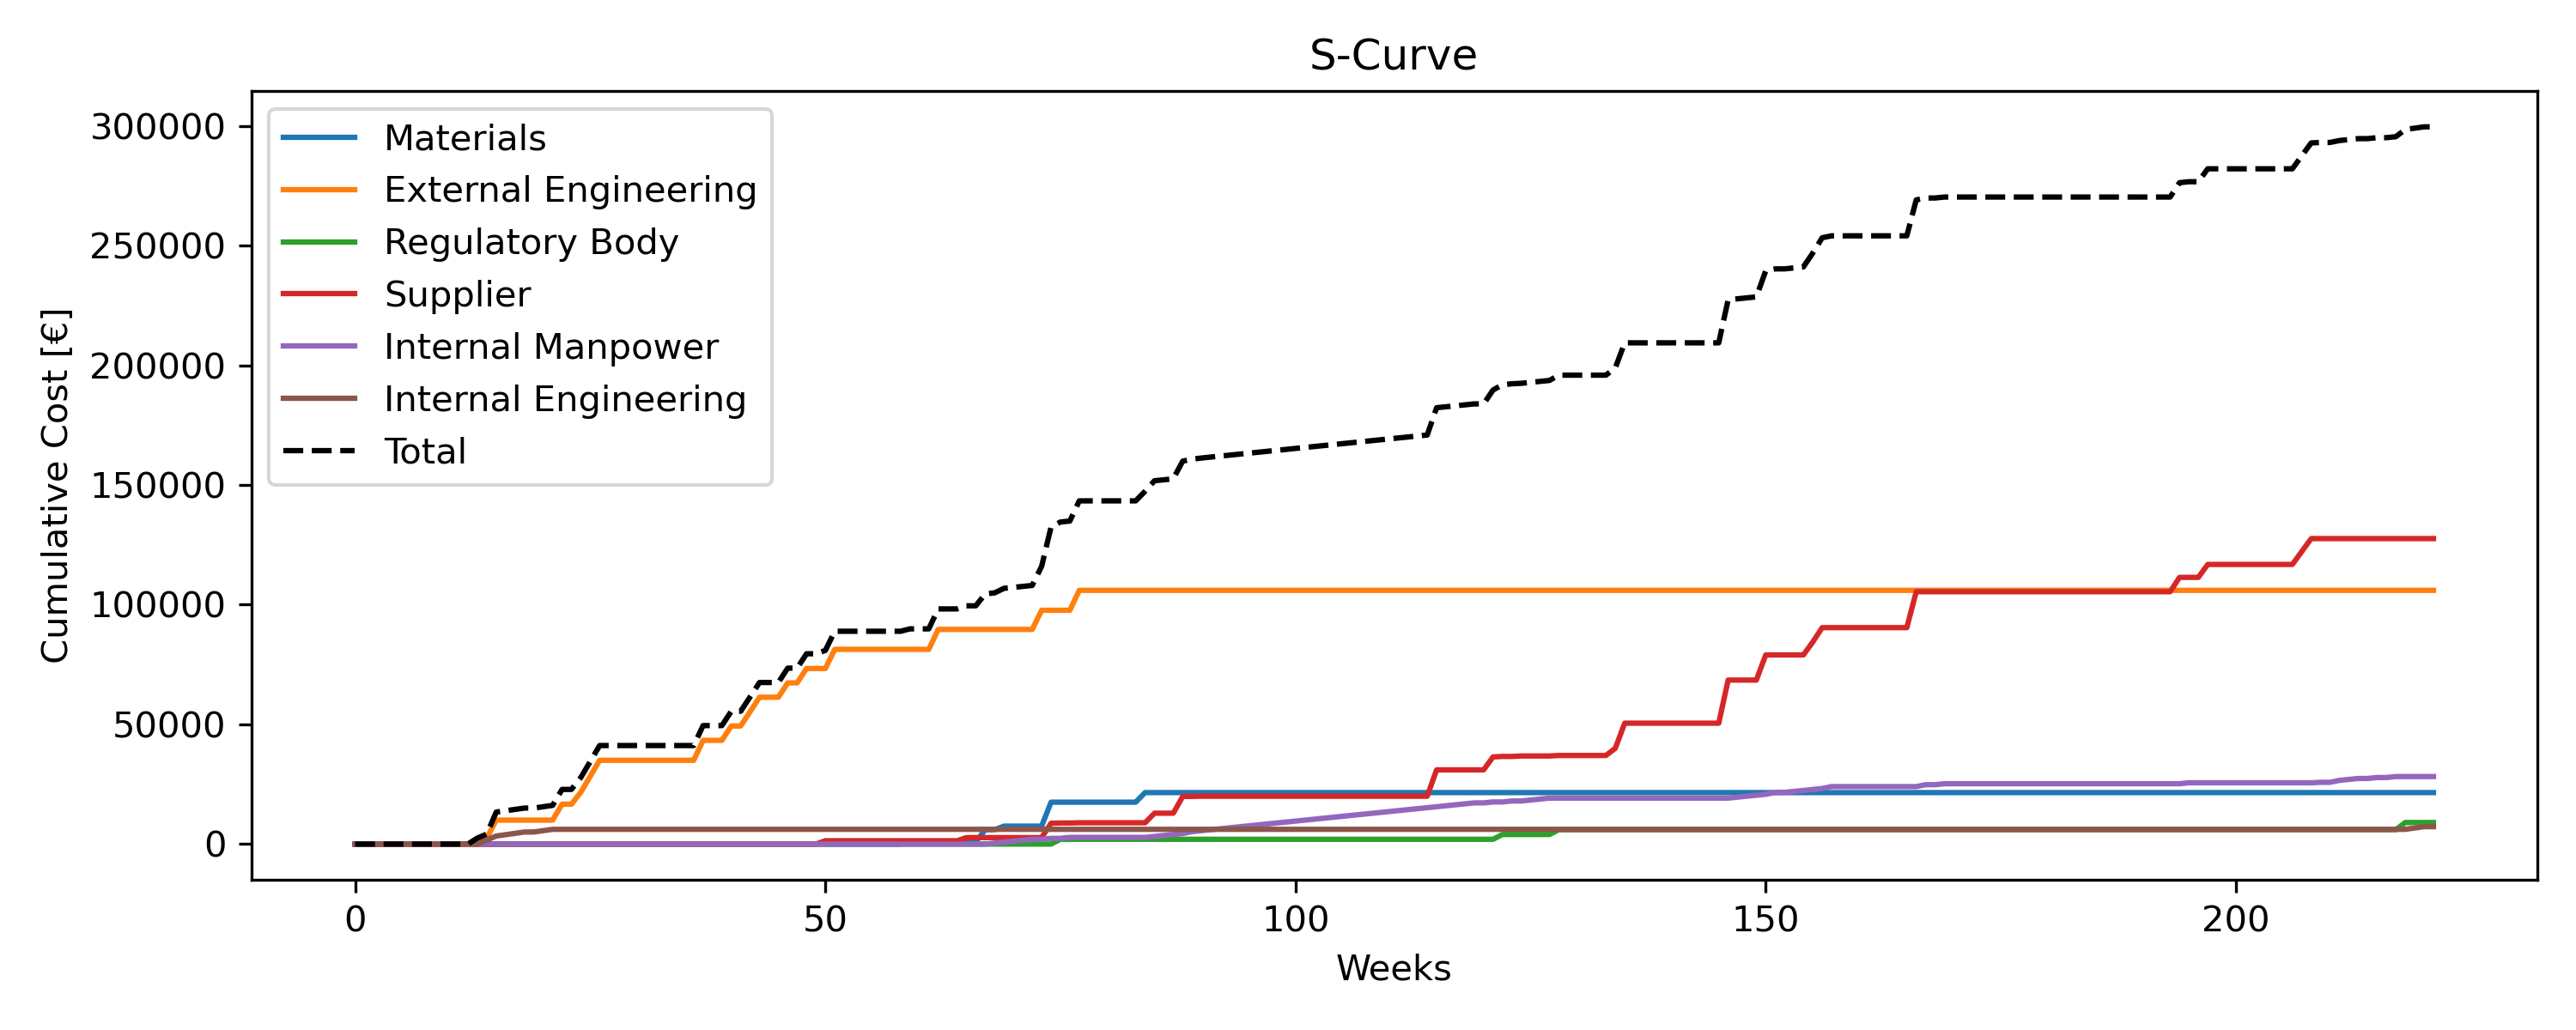
\includegraphics[width=\textwidth]{../s_curve_E.png}
        \captionof{figure}{S-curve - Early Start Scenario}
        \label{fig:scurve_early}
    \end{minipage}\hfill
    \begin{minipage}{\textwidth}
        \centering
        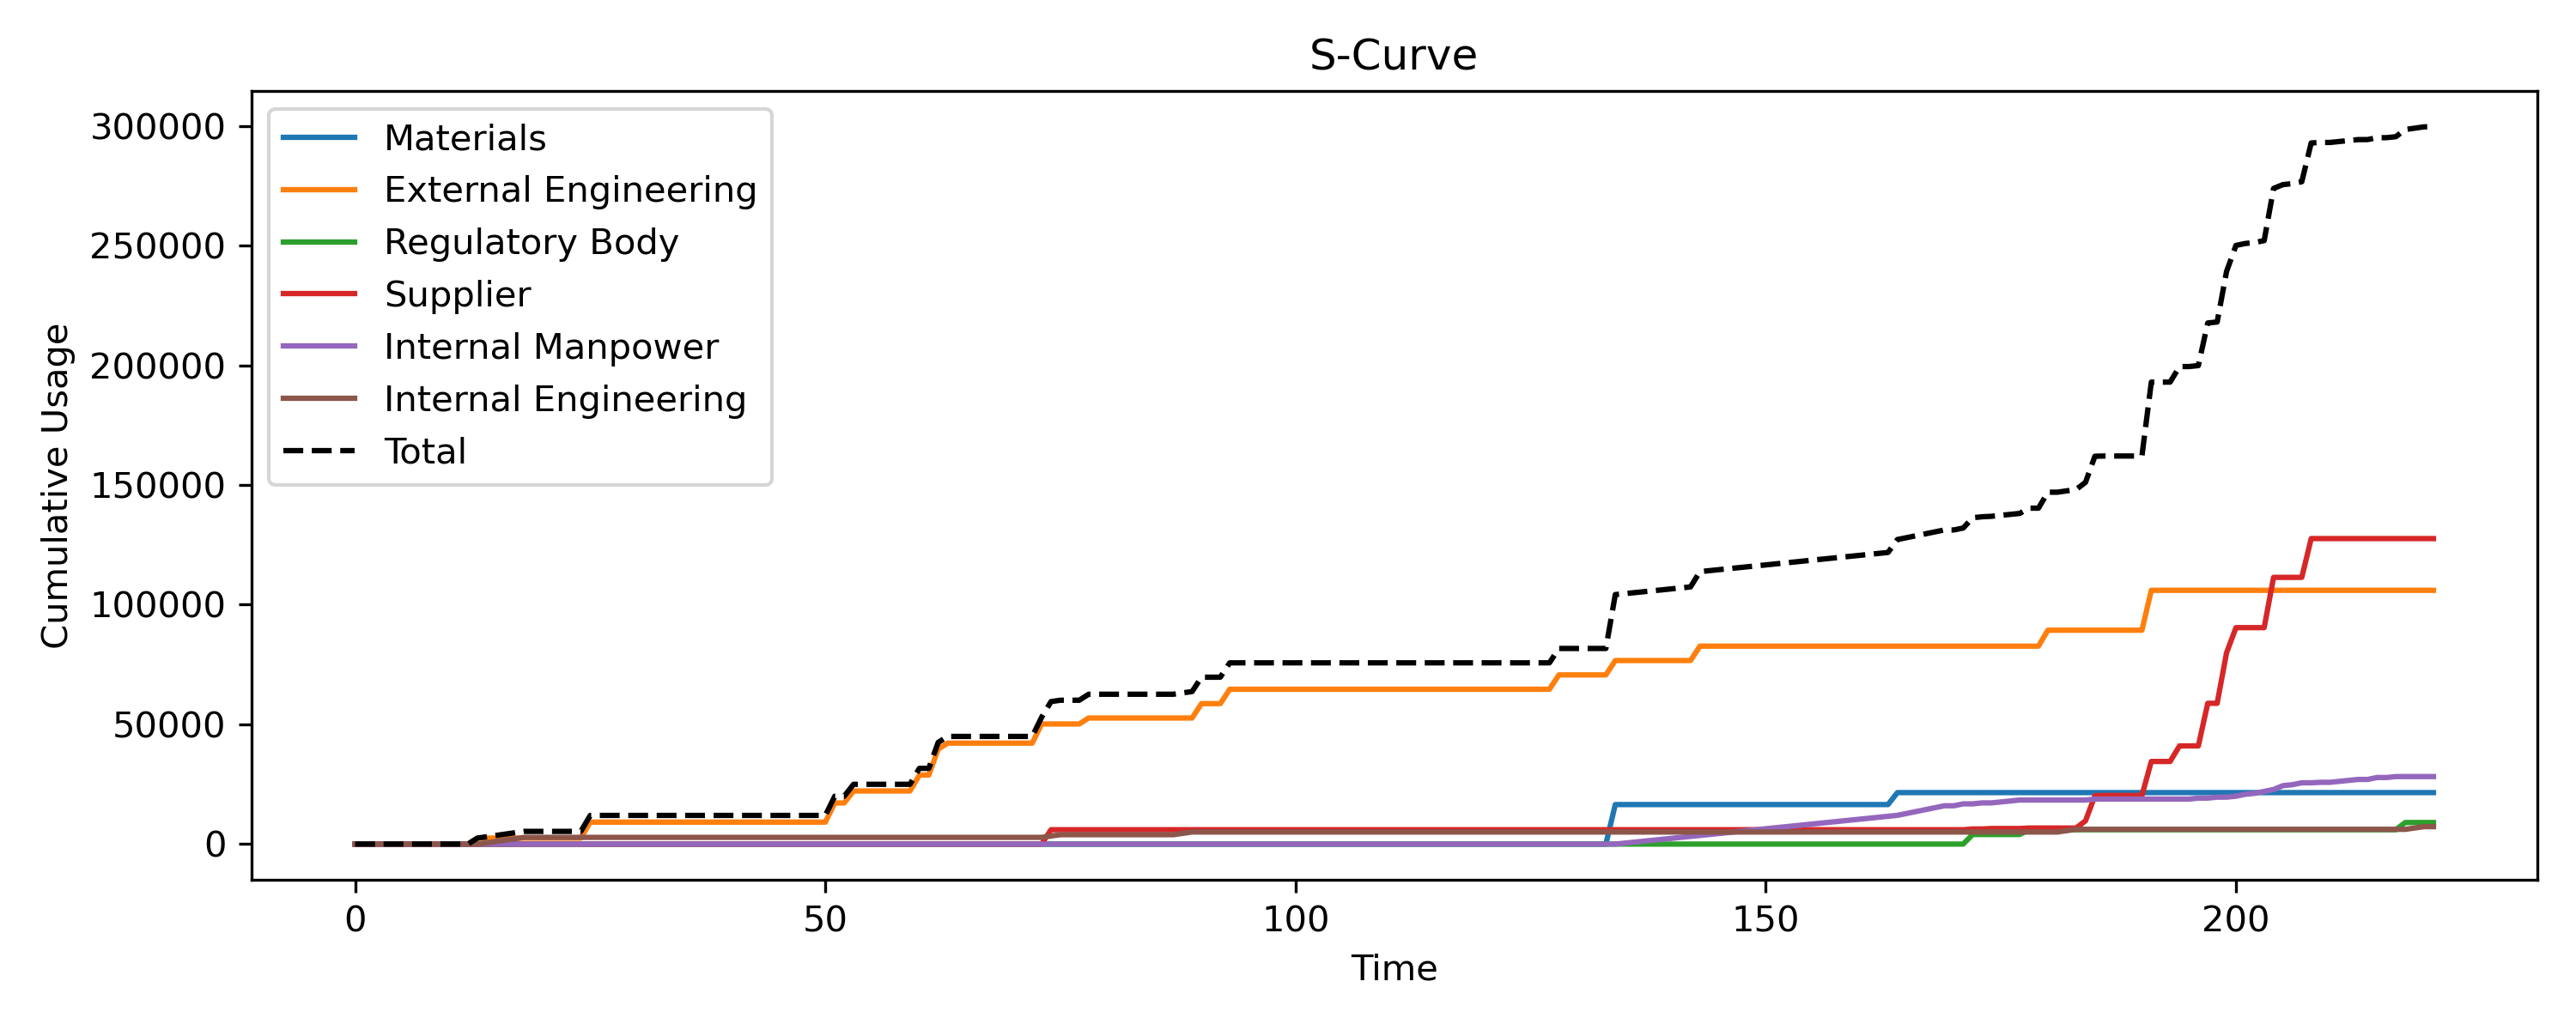
\includegraphics[width=\textwidth]{../s_curve_L.png}
        \captionof{figure}{S-curve - Late Start Scenario}
        \label{fig:scurve_late}
    \end{minipage}
\end{figure}


\section{Cash Flow and Project Balance}
As previously stated, internal costs are allocated continuosly in time while external resource are paid in lump sums, more specifically:
\begin{itemize}
    \item If the cost is lower then 7,500.00 €, the cost is allocated at the delivery.
    \item if the cost is higher then 7,500.00 €, 50\% of the sum is paid upfront and 50\% at delivery.
\end{itemize}

To mitigate financial strain, the modification of the supplier payment structure from the 50\%-50\% split (upfront and at delivery) to a more back-loaded scheme (e.g., 30\% upfront, 70\% at delivery) can be considered.
This adjustment could significantly reduce early cash outflows while maintaining supplier commitment.

A detailed cash flow analysis was carried out to assess the financial feasibility and sustainability of the project across its duration. The following payment scheme for the project's delivery is assumed:
\begin{itemize}
    \item 20\% at the beginning of the project.
    \item 40\% at the midterm, most likely following a review of the progress with the client.
    \item 40\% at the end of the project.
\end{itemize}

The resulting cashflow is hereby represented:

\begin{figure}[H]
    \centering
    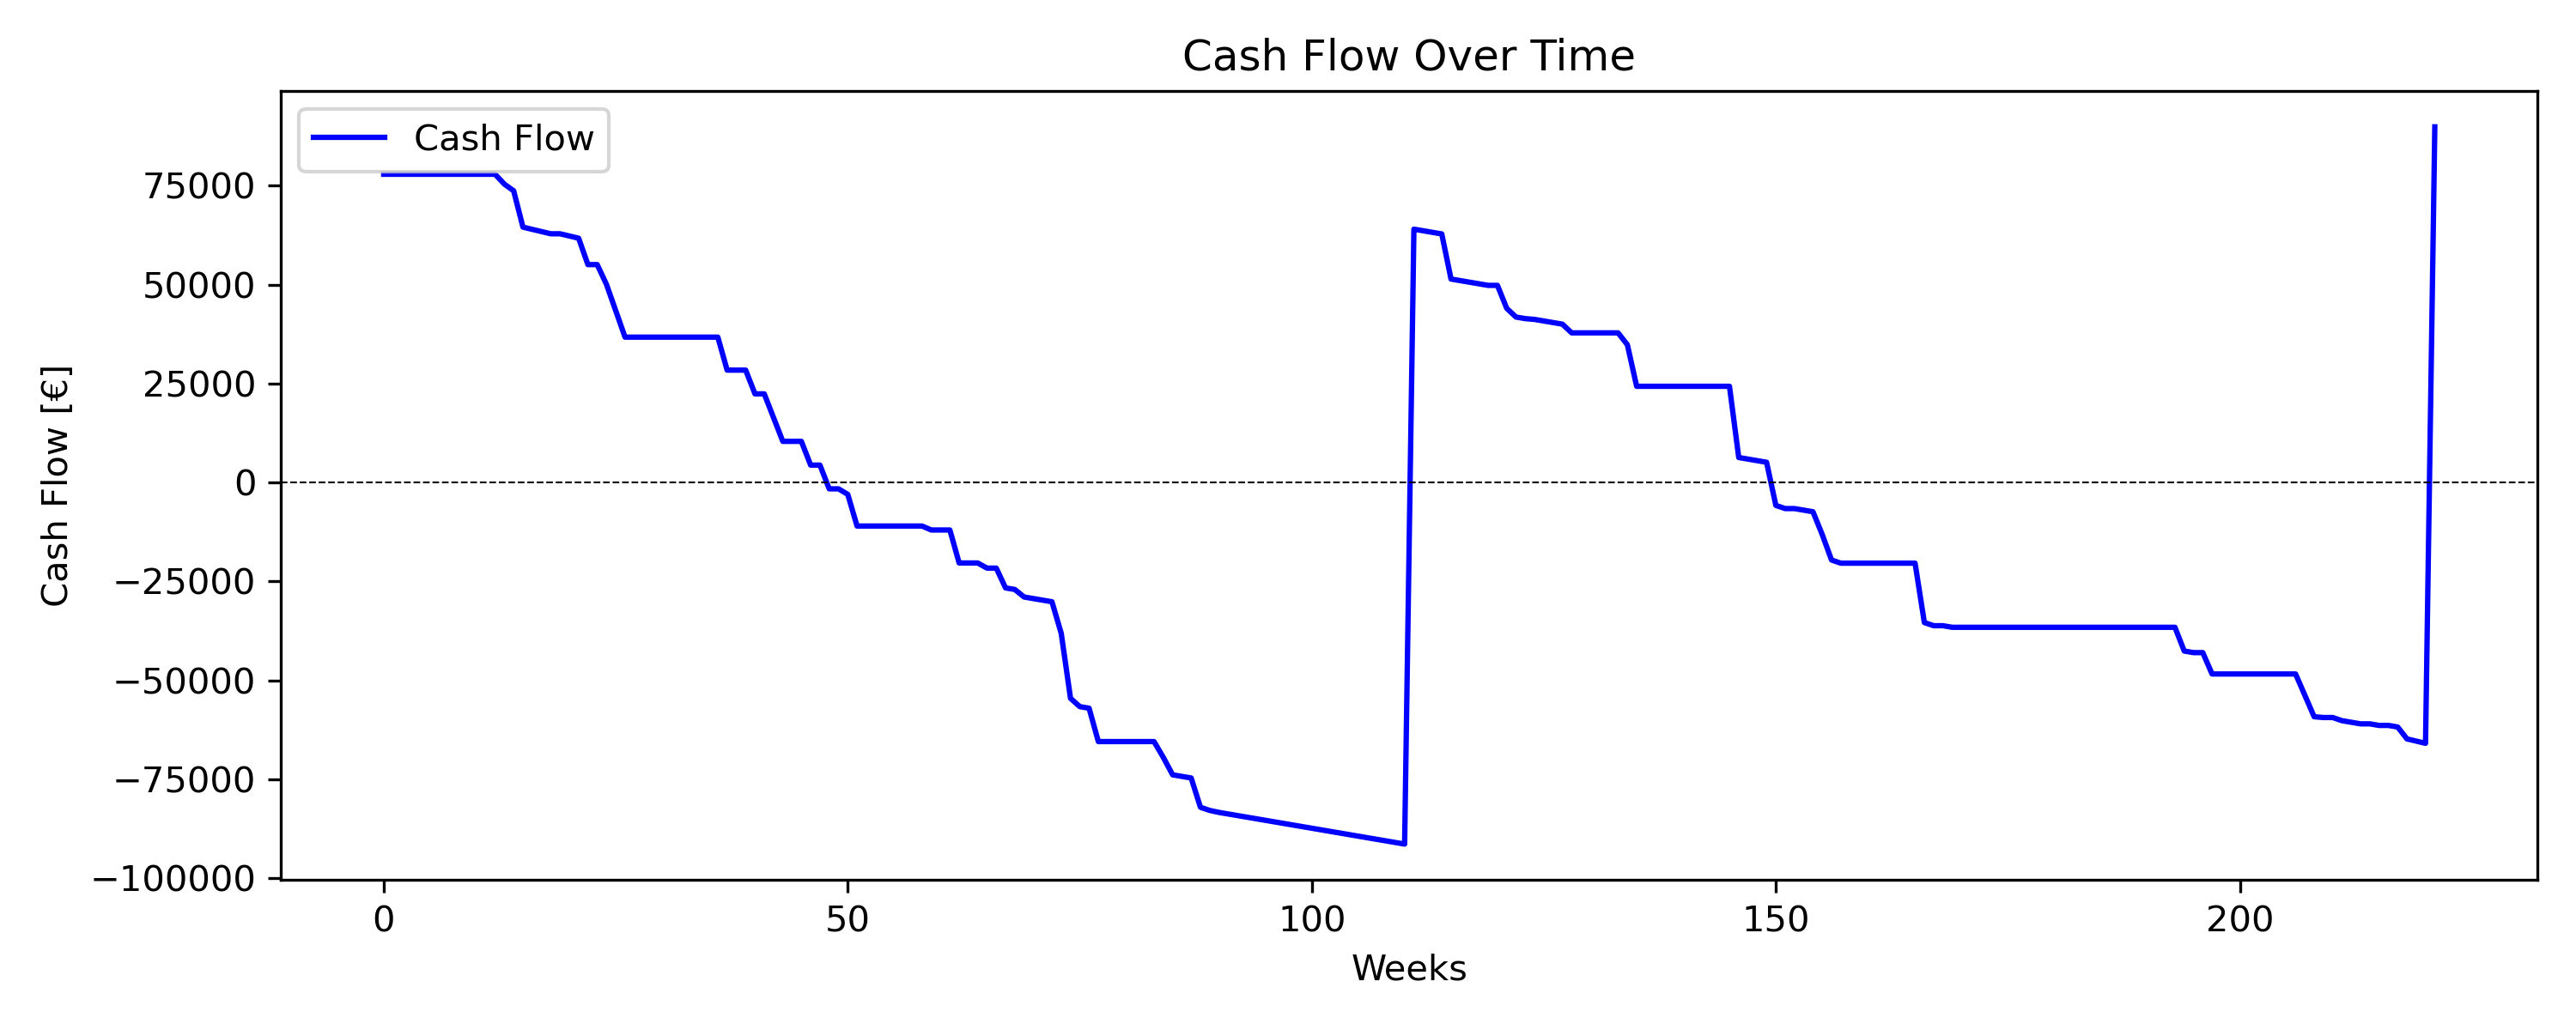
\includegraphics[width=\textwidth]{../cash_flow_E.png}
    \caption{Cash Flow - Early Start Scenario}
    \label{fig:cashflow_early}

\end{figure}
\begin{figure}[H]
    \centering
    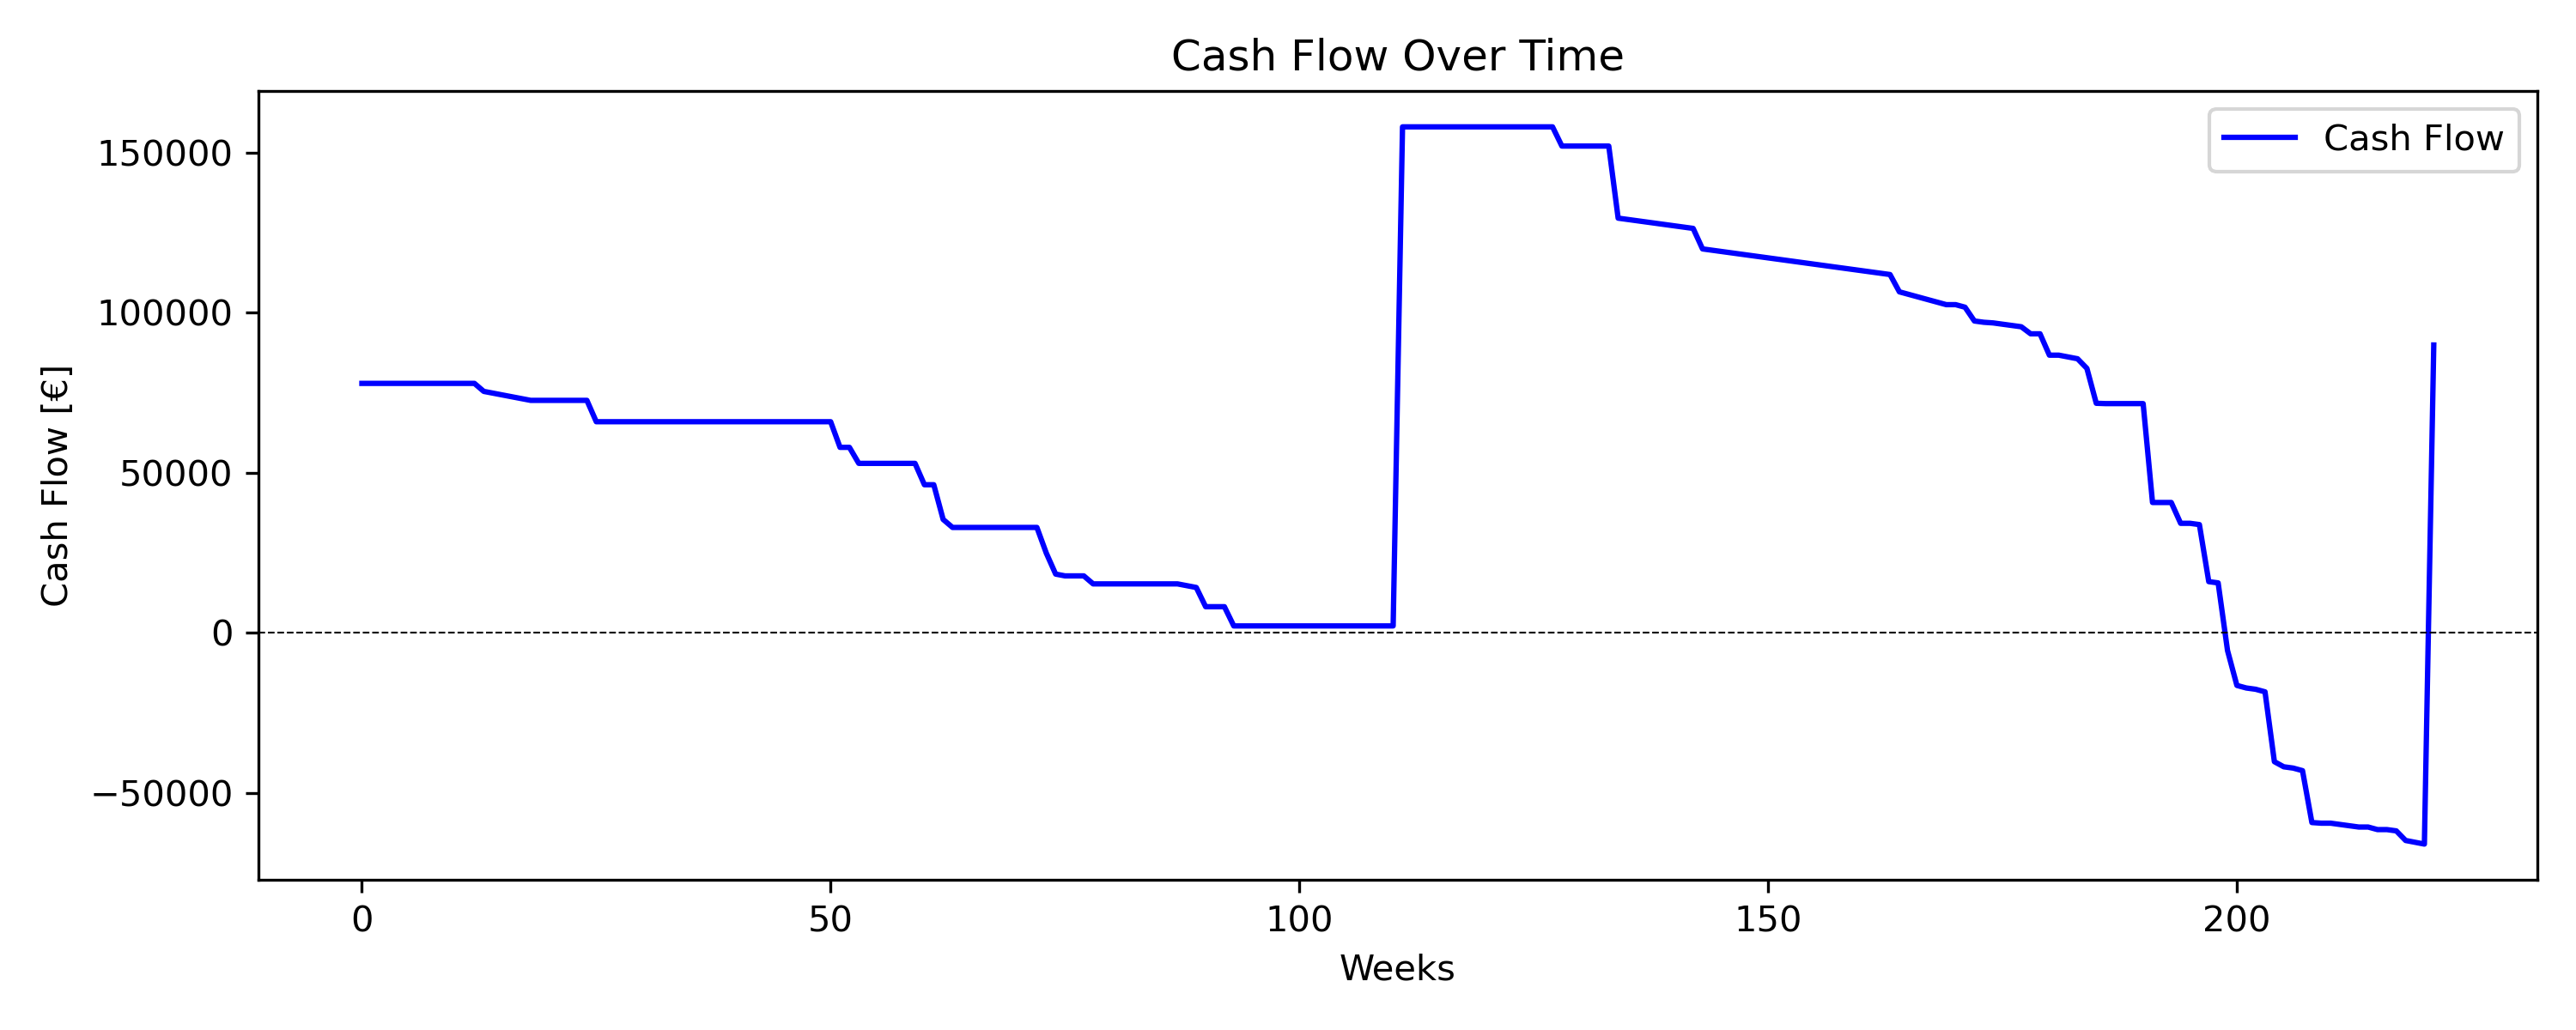
\includegraphics[width=\textwidth]{../cash_flow_L.png}
    \caption{Cash Flow - Late Start Scenario}
    \label{fig:cashflow_late}
\end{figure}

The analysis of the cashflow showed that the project would benefit from a more regular payment structure. Therefore, a set of potential milestones was identified to support a more consistent payment schedule:
\begin{itemize}
    \item Production of 3D model and drawing, that could be shown to the client for approval before components' ordering.
    \item Logic map definition and feedback from the client, before committing to the control system and ordering the flow computer.
    \item Structure assembly completion (to ensure adequacy of the skid with the client), before painting and instrumentation installation.
\end{itemize}

\subsection{Project Balance}
WHAT

\section{Risk Management}

The risk management for the project was conducted using a structured, quantitative approach. The core of the method relied on the calculation of a Project Classification Index (IC), which integrates three key impact areas: Economic (IE), Strategic (IS), and Risk (IR). Each of these dimensions was assessed in terms of impact, with the final index computed as:
IC = (IE × PIE) + (IS × PIS) + (IR × PIR).

The risk identification and evaluation phases produced a categorization into four main areas:
\begin{itemize}
    \item \textbf{TR - Technical risks:} errors in engineering deliverables, design rework.
    \item \textbf{PR - Procurement risks:} supplier delays, component unavailability.
    \item \textbf{CR - Construction risks:} site conditions, labor productivity issues.
    \item \textbf{MR - Managerial risks:} coordination failures, scope creep.
\end{itemize}

andandand RICORDARSI DI METTERE IL CODICE DELLA RISK AREA NELLA TABELLA PER I RISK ITEM NELL'EXCEL

Each identified risk was evaluated based on its probability of occurrence and potential impact, along with the possibile mitigation strategies and their respective cost.
The complete risk register is available in the attached file.

INSERIRE REFERENCE QUI E UN ESEMPIO DELLA TABELLA NELL'EXCEL

This comprehensive analysis allowed for a precise and informed mitigation plan organization and contingency management.
The elected action for each risk item is either:
\begin{itemize}
    \item Accept: accept the risk and its consequences.
    \item Transfer: shift the negative impact to a third party. Usually involves the payment of a risk premium.
    \item Mitigate: reduce the probability of the adverse event. Usually has a cost.
\end{itemize}

Contingency amounts, distributed across the relevant Work Breakdown Elements (WBEs), were determined under the assumption that any risk item with a probability of occurrence greater than 70\% would require full impact allocation as contingency.

Risk monitoring would be conducted periodically throughout execution, with the possibility of introducing corrective actions or updated contingency plans when necessary. This ensures that risk management remains a continuous and adaptive process.

\section{Progress Evaluation}

Progress evaluation is designed to ensure timely monitoring, early detection of deviations, and proactive corrective actions. The structure of the plan supports tracking at the Work Package (WP) level, with progress assessed based on both physical completion and resource consumption.

Key metrics that can be employed for progress tracking include:

1.   Percentage of completion per WP, updated based on:
\begin{itemize}
    \item Milestone: completion is assessed at key project milestones.
    \item 0/100: a binary approach where completion is either 0\% or 100\%.
    \item 50/50: a phased approach where 50\% completion is assessed at midterm reviews.
    \item Level of effort: tracking based on the amount of work completed relative to the total effort.
\end{itemize}

2.   Planned vs. Actual Timeline Comparison, using Gantt chart overlays

3.   Earned Value Analysis (EVA) indicators such as:

SPI / CPI: schedule and cost performance indices.

CV (Cost Variance):

SV (Schedule Variance):

EAC (Estimate at Completion):

ETC (Estimate to Complete):

TCPI (To Complete Cost Performance Index):

In addition, "control checkpoints" were defined at the end of major project phases (e.g., end of engineering, procurement, mechanical erection), enabling formal milestone reviews and progress validation.

The early identification of float in the schedule also offers flexibility: in case of delays in non-critical tasks, corrective actions can be prioritized without impacting the overall project duration.

Regular progress updates would be conducted through weekly or bi-weekly reviews with the responsible OBS units, ensuring alignment between planning and execution throughout the project lifecycle.

\section{Close-Out}

The project close-out phase is structured to ensure a controlled and verifiable conclusion of all planned activities. It includes both technical and administrative procedures required to formally complete the project, deliver final outputs, and transfer responsibility to the client or end-user.

Close-out begins with a comprehensive review of completed deliverables against the original scope, using predefined acceptance criteria. This ensures that all outputs conform to expected quality levels and contractual obligations. Special attention is given to testing-related activities such as Factory Acceptance Tests (FATs), dimensional checks, and non-destructive testing (NDT), which serve as key verification milestones for both structural and process components.

Documentation is a critical part of the close-out phase. A complete Documentation Pack is prepared, including design files, test reports, certificates, and any as-built documentation. This package supports future maintenance, regulatory compliance, and operational readiness.

From a managerial perspective, the close-out process includes:
\begin{itemize}
    \item Final resource and cost alignment.
    \item Compilation and archiving of lessons learned documentation, including questionnaires, etc.
    \item Formal closure of procurement contracts and outstanding obligations.
    \item Internal reviews with all functional units to capture feedback and improvement opportunities.
    \item Preparation and handover of the complete project documentation pack to the client.
    \item Administrative closure and release of project resources.
\end{itemize}

Only after formal acceptance and administrative closure will the project be considered fully concluded. This approach ensures transparency, traceability, and organizational learning for future projects.

\section{Conclusions}
The project underscored the value of traditional project management methods, particularly the importance of a well-defined Work Breakdown Structure (WBS) before scheduling and cost estimation. Different WBS perspectives enhanced clarity and revealed errors, while accurate assumptions were vital for effective planning.
The project demonstrated the application of traditional techniques in a semi-real industrial scenario, resulting in a coherent and executable plan. Using multiple WBS structures and detailed breakdowns provided a comprehensive project view, improving control and traceability.


\subsection{Agile methodology in PW development}
Although the overall organization of the project itself followed a traditional Waterfall approach, appropriate for representing the complete lifecycle of an industrial system, Agile working methods were adopted within the students' team during the development phase.
With fixed delivery deadlines and clearly defined resources (e.g., our personal effort, availability and time), Agile principles were applied by adapting the scope and content of the deliverables to fit these constraints. Key Agile practices included frequent team meetings that served as iterative checkpoints, allowing to incrementally build the final report.
At each stage, progress was reviewed, errors were identified and corrected, and the approach was adjusted accordingly.
Moreover, a Kanban Board was used to identify, assign, plan and monitor the different tasks to complete. The software "YouTrack" served as support.
This incremental and adaptive process enhanced both the quality of our deliverables and our ability to collaborate effectively under time constraints, closely mirroring the behavior of Agile frameworks.

